\documentclass[10pt,a4paper]{article}
\usepackage[utf8]{inputenc}
\usepackage{amsmath}
\usepackage{amsfonts}
\usepackage{amssymb}
\usepackage{mathtools}
\usepackage{parskip}


\DeclareRobustCommand{\bbone}{\text{\usefont{U}{bbold}{m}{n}1}}
\DeclareMathOperator{\EX}{\mathbb{E}}% expected value

\DeclarePairedDelimiterX{\infdivx}[2]{(}{)}{%
  #1\;\delimsize\|\;#2%
}
\newcommand{\infdiv}{D\infdivx}
\newcommand{\infdivlb}{D_{lb}\infdivx}
\DeclarePairedDelimiter{\norm}{\lVert}{\rVert}


\usepackage{graphicx}
\usepackage[left=2cm,right=2cm,top=2cm,bottom=2cm]{geometry}
\author{Gregory A. Ross}

\title{Upper and lower bounds to the marginal likelihood}
\begin{document}


\newcommand{\myrightarrow}[1]{\xrightarrow{\makebox[2em][c]{$\scriptstyle#1$}}}‌


\maketitle
\begin{abstract}
On estimating Bayesian marginal likelihoods using lower and upper bounds. The maximum value of the marginal likelihood is found to be independent of the model and the property of the data.\\

Present an easy to calculate lower bound (mean deviance over the prior), a straightforward way to calculate an upper bound (mean deviance over the posterior), and a tighter version of this upper bound by estimation of the information gain. 
\end{abstract}

\section{Introduction}

Overview and purpose of model comparison
\begin{itemize}
\item The goal is to find the model with the largest marginal likelihood.
\item Like with the AIC, we assume the data has been generated by some true, unknown, distribution.
\end{itemize}


How people estimate marginal likelihoods and Bayes Factors
\begin{itemize}
\item Bos2002Compariosn ACTUALLY CONTAINS COMPARISONS OF APPROXIMATION METHODS - MINE IS PROBABLY BEST
\item BIC and Laplace approximation remain popular in statistics
\item But BIC completely ignores priors. 
\item BIC provides regularizarion based on the number of parameters, but not on the restriction they provide on phase space. This kind of regularization is super useful, e.g. GWAS studies.
\item Statistical physics is often concerned with calculating numerically or analytically normalization constants called partition functions.
\item In my field (biomolecular chemistry?) and medicinal chemistry, complicated and advanced methods have been codified and are available on lots of software.
\end{itemize}

The point of this work is come up with practical methods for Bayesian model selection by considering bounds on the marginal likelihoods. 
\begin{itemize}
\item The success of the DIC is that it is easily computable from MCMC data - we'll strive for that ease of use.
\item From the conclusion of the original paper, after the critcisms: "DIC instead addresses how well the posterior might predict future data generated by the same mechanism that gave rise to the observed data; this posterior predictive outlook might be considered intuitively more appealing in many practical contexts.". I believe this intuition is achieved by the upper bound.
\end{itemize}

Complexity is a combination of non-linearity of the functional form of the model and the regularizing ability of the priors. Something that the authors of the DIC are aware of. 

Read and check through "Aikin1991Posterior", which considers the posterior mean of the likelihood (not log likelihood) for model comparison.


Read and check through "Oladyshkin2019Connection.pdf" to see if I've been scoped in anyway.
\begin{itemize}
\item Equation 18 (page 8) actually has the basis to derive my upper bound. They don't seem to be aware of what they have though.
\end{itemize}
\section{Background}

\subsection{Marginal Likelihoods and Bayes Factors}
We have a set of models, indexed by $m$, and each has it's own parameter space. The goal is either select the best model or the best way to aggregate predictions over the models. 
State Bayes theorem and introduce the marginal likelihood/evidence.
\begin{align}
p_m(\theta | X) =  \frac{p_m(X|\theta) p_m(\theta)}{ \int p_m(X|\theta) p_m(\theta) \, d\theta}
\end{align}
Will drop the subscript $m$ when not considering multiple models.
The marginal likelihood is a "consistent" estimator for model selection or whatever, but is normally too difficult to calculate properly. 
\begin{align}
\mathcal{L}_m(X) = \log \int p(X|\theta) p(\theta)  \, d\theta,
\end{align}
The weighting attributed to model $m$ is proportional to $\exp(\mathcal{L}_m(X))$.
\begin{itemize}
\item Bayes factors are great because of blah blah
\item Bayes factors are bad because dependence on prior, proper priors requred, require software infrastructure over and above that required to estimate the parameters.
\item etc etc
\item which is why people frequently use information criteria instead.
\end{itemize}

\subsection{Information criteria}
Marginal likelihoods and Bayes factors are difficult to calculate and people sometimes don't want to calculate them anyway. Information criteria are used for quick and easy model selection. They frequently take the form
\begin{align}
IC  = \log p(D|\theta_{IC}) + P_{IC}
\label{eq:inf_crit}
\end{align}
Where $\theta_{IC}$ is the parameter estimate and $P$ is term that penalizes for the number of free parameters. 
\begin{itemize}
\item For the AIC, $\theta_{IC}$ is the maximum likelihood estimate and $P$ is the number of free parameters. [How is this motivated?]
\item For the BIC, $\theta_{IC}$ is the frequently taken to be the mean, although the original paper didn't make this clear and $P_{BIC}$ is $k\log N$.
\item In the DIC, $\theta_{IC}$ is the frequently taken to be the posterior mean, although the original paper didn't make this clear and $P_{BIC}$ is blah blah with different embelishments such as blah blah... [How is this motivated?]
\end{itemize}

\section{Theoretical results}
\subsection{Bounding the marginal likelihood}

Motivate the approach here: MCMC friendly and straightforward.

Re-arrange Bayes' theorem in form that yields both the upper and lower bounds.
\begin{align}
\mathcal{L}(X) &= \log p(X | \theta) - \log \frac{p(\theta | X)}{p(\theta)} \label{eq:logmarglike}\\
&= \int \left [ \log p(X | \theta) -  \log \frac{p(\theta | X)}{p(\theta)} \right ] p(\theta|X) \, d\theta  \notag\\
&=\EX_{\theta | X} [ \log  p(X|\theta)]  -  \infdiv[\big]{p(\theta | X)}{p(\theta)},
\label{eq:marg_up}
\end{align}
As long as one can sample from the posterior, the likelihood term, $\EX_{\theta | X} [ \log  p(X|\theta)]$, is trivial to estimate. However, the KL divergence $ \infdiv[\big]{p(\theta | X)}{p(\theta)}$ may be difficult to calculate, particular so if $k$ is large. Instead, one could exploit the non-negativity of the KL divergence to arrive at trivial upper bound to the log marginal likelihood
\begin{align}
\mathcal{L}(X) \leq \EX_{\theta | X} [ \log  p(X|\theta)].
\end{align}
A tighter bound can be obtained if one uses an easily computable lower bound to the KL divergence. Defining $\infdivlb[\big]{p(\theta | X)}{p(\theta)}$ such that it is less than or equal to $\infdiv[\big]{p(\theta | X)}{p(\theta)}$, we have
\begin{align}
\mathcal{L}(X) \leq \EX_{\theta | X} [ \log  p(X|\theta)] -  \infdivlb[\big]{p(\theta | X)}{p(\theta)}
\end{align}
Different ways to compute $\infdivlb[\big]{p(\theta | X)}{p(\theta)}$ will be explored later in the paper.

A lower bound to the log marginal likelihood can be obtained if express equation \ref{eq:logmarglike} as an expectation over the prior rather than the posterior:
\begin{align}
\mathcal{L}(X) &= \EX_{\theta} [ \log  p(X|\theta)] + \infdiv[\big]{p(\theta)}{ p(\theta|X)} \notag\\
&\geq  \EX_{\theta} [ \log  p(X|\theta)] 
\end{align}
The likelihood term is even easier to estimate than above because sampling over the prior. In the vast majority of cases, the prior is easy to sample from or one already has samples from the prior (from Bayesian updating). Nonnegativity of KL divergence yields
\begin{align}
\mathcal{L}(X) \geq \EX_{\theta } [ \log  p(X|\theta)] 
\end{align}
In most circumstances, this won't be as tight as before because prior is broader - gaussian example. As above, we can construct a tighter lower bound by lower bounding the KL divergence:
\begin{align}
\mathcal{L}(X) \geq \EX_{\theta | X} [ \log  p(X|\theta)] + \infdivlb[\big]{p(\theta | X)}{p(\theta)}
\end{align}

The utility of these bounds will be explored with numerical examples.
\subsubsection{The absolute upper bound to marginal likelihood}
To put these bounds in context...

It is under appreciated that the entropy of the data generating process is an absolute upper bound to the log marginal likelihood in the limit of infinite data. 
\subsection{The KL divergence as the number of free parameters}
In this form, the log marginal likelihood has the form of an information criterion, with a likelihood term and the KL divergence between the posterior and prior playing the role of the effective number of free parameters. Intuitively, the greater the degree of change between the prior and posterior, the more ``free'' the parameters were. 

The interpretation of the KL divergence in equation \ref{eq:marg_up}  as the effective number of free parameters can be made rigorous by considering the limit of infinite data. In this limit [SEE GELMAN CH 4 AND EVERNOTE "Asymptotically we are all dead" FOR SPECIFIC CONDITIONS] the posterior density tends towards a normal distribution
\begin{align}
%\lim_{n\rightarrow\infty }p(\theta|X^n) = N \big (\theta_0, (n I(\theta_0))^{-1/2} \big) \\
%p(\theta|X^n) \myrightarrow{L^1} N \big (\theta_0, (n I(\theta_0))^{-1/2} \big) \\
p(\theta|X^n) \rightarrow N \big (\theta_0, (n I(\theta_0))^{-1/2} \big),
\end{align}
where the convergence can be described in various senses [bayesian procedures ch12, Clarke1999Asymptotic,  and references in Johnstone2010High]. [Relative entropy between posterior and the above tends to zero, see Clarke1999Asymptotic] which, in the same limit, tends towards the delta distribution
\begin{align}
\lim_{n\rightarrow\infty } N \big (\theta_0, (n I(\theta_0))^{-1/2} \big) = \delta(\theta - \theta_0)
\end{align}


 For the likelihood term in equation \ref{eq:marg_up}, we have
\begin{align}
\lim_{n\rightarrow\infty }\EX_{\theta | X^n} [ \log  p(X^n|\theta)]  &= \int \delta (\theta - \theta_0) \log  p(X^n|\theta) \, d\theta \notag\\
&= \log  p(D|\theta_0).
\end{align}
For KL divergence term
\begin{align}
\lim_{n\rightarrow\infty } \infdiv[\big]{p(\theta | X^n)}{p(\theta)} &= \lim_{n\rightarrow\infty } \left [ -H(\theta|D) - \int p(\theta|D) \log p(\theta) \, d\theta \right] \notag\\
&= \frac{1}{2} \log \left( (2\pi e n)^k  |I(\theta_0)|^{-1}\right) + \log p(\theta_0) \notag\\
&=  \frac{1}{2} k\log n + \mathcal{O}(1) 
\end{align}
Meaning that the KL divergence between the posterior and the prior asymptotically tends towards the penalizing term in the BIC.

It should not be surprising that we recover the BIC in the asymptotic data limit since equation \ref{eq:marg_up} is an exact expression for the log-marginal likelihood. What should be interesting is this limit is consistent with our interpretation that the KL divergence is the effective number of parameters. Importantly, this interpretation is valid for data sets with a finite, rather than asymptotic, amount of data.

Alternatively, we can express the log marginal likelihood as an expectation over the prior:
\begin{align}
L(D) &= \log p(D | \theta) + \log \frac{p(\theta)}{p(\theta | D)}  \notag\\
&= \EX_{\theta} [ \log  p(D|\theta)] + \infdiv[\big]{p(\theta)}{ p(\theta|D)}
\end{align}
This expression also has a form reminiscent of the an information criterion


From the non-negativity of the KL divergence, we have the following bounds
\begin{align}
\EX_{\theta} [\log  p(D|\theta)  ] \leq L(D) \leq \EX_{\theta | D} [ \log  p(D|\theta) ]
\label{eq:upp_low}
\end{align}
This also has the form of an information criterion, but 

One of the main focuses of this work is to assess utility and interpretation of these bounds.

These bounds are very easy to calculate as usually one has either samples of the prior or can generate samples. It's already assumed that practitioners have samples from the posterior, and are trying to get an idea of model quality.

Intuitively, one would expect the upper bound to be tighter than the lower bound because $p_m(D|\theta)$ is in the denominator in $D(p_m(\theta) || p_m(D|\theta)$. The KL divergence could blow up if the posterior more tightly peaked than the prior: there could be large volumes where the prior is much larger than the posterior. Although the relative tightness of either bound would depend on the actual distributions. This intuition is true in the case of two Gaussian distributions with the same mean but different standard deviations.
\subsection{Tightness of bound with Gaussian distributions}
The KL divergence between two Gaussian distributions, indexed with $i$ and $j$ is given by 
\begin{align}
\infdiv[\big]{i}{j} = \log\frac{\sigma_j}{\sigma_i} + \frac{\sigma_i^2 + (\mu_i - \mu_j)^2}{2\sigma_j^2} - \frac{1}{2},
\end{align}
where $\mu$ and $\sigma$ are the mean and standard deviation, respectively. Let the index 1 denote the prior and index 2 denote the posterior. As it is often the case that the prior is broader than the posterior, let us define $r = \sigma_1 / \sigma_2$ with $r \geq 1$. The relative tightness of the upper and lower bounds in equation \ref{eq:upp_low}  is determined by the sign of the difference
\begin{align}
\Delta := \infdiv[\big]{1}{2} - \infdiv[\big]{2}{1}.
\end{align}
For the upper bound to be as least as tight as the lower bound, we require that $\Delta \geq 0$. Writing $\Delta$ in terms of $r$ immediately reveals that
\begin{align}
\Delta &= -\log r^2 + \frac{1}{2}r^2 - \frac{1}{2}r^{-2}  + \frac{1}{2}(\mu_1 -\mu_2)^2\left(\frac{1}{\sigma_2^2} - \frac{1}{\sigma_1^2}\right) \\
& \geq -\log r^2 + \frac{1}{2}r^2 - \frac{1}{2}r^{-2},
\end{align}
since $\sigma_1 \geq \sigma 2$. To proceed, we will use the fundamental upper bound $\log x \leq x -1$:
\begin{align}
\Delta &\geq -\log r^2 + \frac{1}{2}r^2 - \frac{1}{2}r^{-2} \\
&\geq (r^2 - 1) + \frac{1}{2}r^2 - \frac{1}{2}r^{-2} \\
&= \frac{1}{2}r^{-2} (3r^4 - 2r^2 -1) \\
&= \frac{1}{2}r^{-2}  (3r^2 +1)(r^2 - 1) \\
&\geq 0,
\end{align}
Since $r \geq 1$. Therefore, in case of a Gaussian prior and a Gaussian posterior, the upper bound of equation $\ref{eq:upp_low}$ is indeed tighter than the lower bound.


\clearpage


\begin{itemize}
\item State the lower and upper bound. The introduction of the KL divergence will be required after one of them has been introduced.
\item Intuitively, one would expect the upper bound to be tighter than the lower bound because $p_m(D|\theta)$ is in the denominator in $D(p_m(\theta) || p_m(D|\theta)$. The KL divergence could blow up if the posterior more tightly peaked than the prior: there could be large volumes where the prior is much larger than the posterior. Although the relative tightness of either bound would depend on the actual distributions.
\item Show/summarize the example of the KL divergence of 2 Gaussians in both directions. If the prior has the larger $\sigma$ and the means are the same, then $D(p_m(\theta) || p_m(D|\theta) \geq D(p_m(D|\theta) || p_m(\theta))$. I have another simple example (which needs checking, that also demonstrates this.]
\item Go into how the KL divergence can be bounded using samples from the prior and posterior. We use the same samples for the KL divergence in the upper and lower bound.
\item Then contextualize these bounds by discussing how each expresses aspects of Occam's razor.
\item Provide further context by relating both the entropy of the true data generating distribution.
\end{itemize}



\subsection{WIP}
Let $L_m(D)$ denote the natural logarithm of the marginal likelihood of a Bayesian model $m$ with data D
\begin{align}
L_m(D) = \log \int p_m(\theta) p_m(D|\theta) d\theta,
\end{align}
where $p_m(\theta) $ is the model prior and $p_m(D|\theta) $ is the likelihood. Capital letters will denote random variables, whereas lowercase letters will denote realisations of the random variables. This note is primarily concerned with regression problems where the data comprises a response variable $Y$ and explanatory variables $X$. In this case, the likelihood has the form $p_m(Y|X, \theta)$.

\paragraph{A weak lower bound can be established by using Jensen's inequality.} If $\psi$ is a concave function and $X$ is a random variable, then Jensen's inequality can be expressed as $\psi(\mathbf{E}[X ] ) \geq \mathbf{E}[\psi(X)]$. As logarithms are concave functions, we immediately have
\begin{align}
L_m(D) \geq \int p_m(\theta) \log  p_m(D|\theta) d\theta 
\label{eq:lb}
\end{align}
This lower bound to $L_m$ can be estimated by sampling from the prior and \emph{not} the posterior. When the prior has an analytic form (such as a normal distribution), this could be very straightforward. The utility of this lower bound will be investigated later on in this note.

\begin{itemize}
\item Although the bound may be weak in practice, it has pedagogical value in demostrating how marginal likelihoods encapsulate Occam's razor.
\item This explaination complements Mackay's eloquent and accessible description.
\end{itemize}



\paragraph{The information gain determines the tightness of the lower bound.} To show this, we'll start by re-expressing the marginal likelihood. From Bayes theorem, we have
\begin{align}
L_m(D) = \log p_m(D | \theta) - \log \frac{p_m(\theta | D)}{p_m(\theta)}
\end{align}
As the the left-hand-side is not a function of $\theta$, we also have
\begin{align}
L_m(D) &=\int  p_m(\theta | D) \log p(D | \theta) \, d\theta - \int  p_m(\theta | D) \log \frac{p_m(\theta | D)}{p(\theta)} \, d\theta \\
&= \mathbf{E}_{\theta|D,m} \left[ \log p_m(D|\theta) \right ]  - D(p_m(\theta | D) || p_m(\theta) ),
\end{align}
where $ D(p_m(\theta | D) || p_m(\theta) )$ is the Bayesian information gain.

Putting this with equation \ref{eq:lb},
\begin{align}
\int p_m(\theta) \log  p_m(D|\theta) d\theta \leq \int p_m(\theta | D) \log p(D | \theta) \, d\theta  - D(p_m(\theta | D) || p_m(\theta) )
\end{align}
So if $D(p_m(\theta | D) || p_m(\theta) )$ is small, then the lower bound is tight. 

\paragraph{Taking the expectation with respect to the prior is far more informative, however.} This gives
\begin{align}
L_m(D) &=\int  p_m(\theta) \log p(D | \theta) \, d\theta + \int  p_m(\theta) \log \frac{p_m(\theta)}{p(\theta | D)} \, d\theta \\
&= \int  p_m(\theta) \log p(D | \theta) \, d\theta + D(p_m(\theta) || p_m(\theta | D) ),
\end{align}
From the nonnegativity of the relative entropy, automatically get the lower bound $L_m(D) \geq \int  p_m(\theta) \log p(D | \theta) \, d\theta$ \emph{and} we know the precise difference: $ D(p_m(\theta) || p_m(\theta | D) )$. If we can lower bound $ D(p_m(\theta) || p_m(\theta | D) )$ then we get an even tighter lower bound for $L_m(D)$.

\paragraph{An upper bound to the log marginal likelihood is easily calculable from MCMC.}  Noting the fact that the KL divergence is greater than or equal to zero, we have the upper bound
\begin{align}
L_m(D) \leq \int  p_m(\theta | D) \log p(D | \theta) \, d\theta
\end{align}

\paragraph{We have tighter upper bound by estimating or bounding the information gain.}
For ease of use following MCMC samples from the posterior, the KL divergence should estimated using methods that are as straightforwards as possible. One can calculate the KL divergence by optimizing a lower bound
\begin{itemize}
\item Nguyen, X., Wainwright, M.J. and Jordan, M.I., 2010. Estimating divergence functionals and the likelihood ratio by convex risk minimization. IEEE Transactions on Information Theory, 56(11), pp.5847-5861.
\item Nowozin, S., Cseke, B. and Tomioka, R., 2016. f-gan: Training generative neural samplers using variational divergence minimization. In Advances in neural information processing systems (pp. 271-279)
\end{itemize}

Or, one can estimate the KL divergence using a classification
\begin{itemize}
\item https://tiao.io/post/density-ratio-estimation-for-kl-divergence-minimization-between-implicit-distributions/
\end{itemize}

\paragraph{Note that I have the usuable inequalities}
\begin{align}
\mathbf{E}_{\theta|m} \left[  \log p_m(D|\theta)  \right ]  \leq L_m(D) \leq  \mathbf{E}_{\theta|D,m} \left[ \log p_m(D|\theta) \right ] \\
\int_\Theta p_m(\theta) \log  p_m(D|\theta) \, d\theta   \leq L_m(D) \leq \int_\Theta p_m(\theta|D) \log  p_m(D|\theta) \, d\theta 
\end{align}
The smaller the information gain, i.e. $D( p(\theta |D) || p(\theta))$, the tighter the bounds. 
\begin{itemize}
\item By analogy with the AIC, BIC, etc, the KL divergence can be considered as the effective number of \emph{free} parameters of the model. The more changeable they are, the more ``free'' they are. 
\item Unlike the lower bound, the upper bound (mean deviance over the posterior) lacks the penalization for the model complexity.
\item The lower bound probably penalizes the complexity too strongly.
\item I have proofs for Gaussians and an example that demonstate that when the prior has a larger width than the posterior, the lower bound KL divergence really is larger.
\item {\textbf{The lower bound penalizes complexity too much, whereas the upper bound does not penalize complexity enough.}} This leads naturally to a section that explains how these bounds are related to Occam's razor.
\end{itemize}

\paragraph{In the large data limit, this lower bound provides an explanation to Occam's razor.} Let the \emph{true} data generating distribution for $X$ and $Y$ be denoted $p_t(X,Y)$ and let the data be composed of $N$ pairs of $Y$ and $X$, such the log-likelihood can be expressed as the sum
\begin{align}
\log p_m(Y|X,\theta)=  \sum^N_{i=1} \log p_m(y_i|x_i,\theta),
\end{align}
then in the large data limit, we find that the likelihood can be expressed as
\begin{align}
\lim_{N \rightarrow \infty} \log p_m(Y|X,\theta) &= N \int p_t(x, y)  \log \big[p_m(y|x,\theta) \big]dx dy \notag\\
&=N \int p_t(x, y)  \log \left[ p_m(y|x,\theta) \frac{p_t(y|x)}{p_t(y|x)} \right] dx dy  \notag\\
&= N  \int p_t(x, y)  \log p_t(y|x) dx dy -N  \int p_t(x, y)  \log \left[  \frac{p_t(y|x)}{p_m(y|x,\theta)} \right] dx dy \notag\\
&= -N H(Y|X) - N D(p_t(y|x) || p_m(y|x,\theta)) ,
\label{eq:asym_like}
\end{align}
where $H(Y|X)$ is the conditional entropy of the true data generating distribution, and $D(p_t(y|x) || p_m(y|x,\theta))$ is the Kullback-Leibler divergence (or, relative entropy) between the true generating distribution and the likelihood for a given value of $\theta$. The above forms the starting point for the Akaike information criterion. Plugging this into equation \ref{eq:lb}, we have
\begin{align}
\lim_{N \rightarrow \infty} L_m(D)  \leq -N H(Y|X) - N \mathbf{E}_{\theta|m} D(p_t(y|x) || p_m(y|x,\theta)),
\end{align}
where $ \mathbf{E}_{\theta|m}$ denotes the expectation with respect to the model prior. From the perspective od model comparison, the best model is one that minimizes $ \mathbf{E}_{\theta|m} D(p_t(y|x) || p_m(y|x,\theta))$. As the KL divergence is always positive, the negative of the conditional entropy $H(Y|X)$ presents an absolute limit that cannot be exceeded by any model. 

The more flexible the model $m$, the lower the value that $D(p_t(y|x) || p_m(y|x,\theta))$ can be for particular value of $\theta$. However, for the most flexible models, the more values of $\theta$ there are that represent terrible fits with large values for $D(p_t(y|x) || p_m(y|x,\theta))$. The expectation of the KL divergence over the prior demonstrates the regularizing effects of the prior. A well chosen prior would limit the volumes of $\theta$ that have very high KL divergences. In the above lower bound, model complexity can be seen a the result of an interplay between the prior and the functional form of the model. A model with a highly complex function form and a scrict prior could achieve the sane value of $\mathbf{E}_{\theta|m} D(p_t(y|x) || p_m(y|x,\theta))$ as a less complex model with a more lenient prior. 

\begin{figure}
\centering
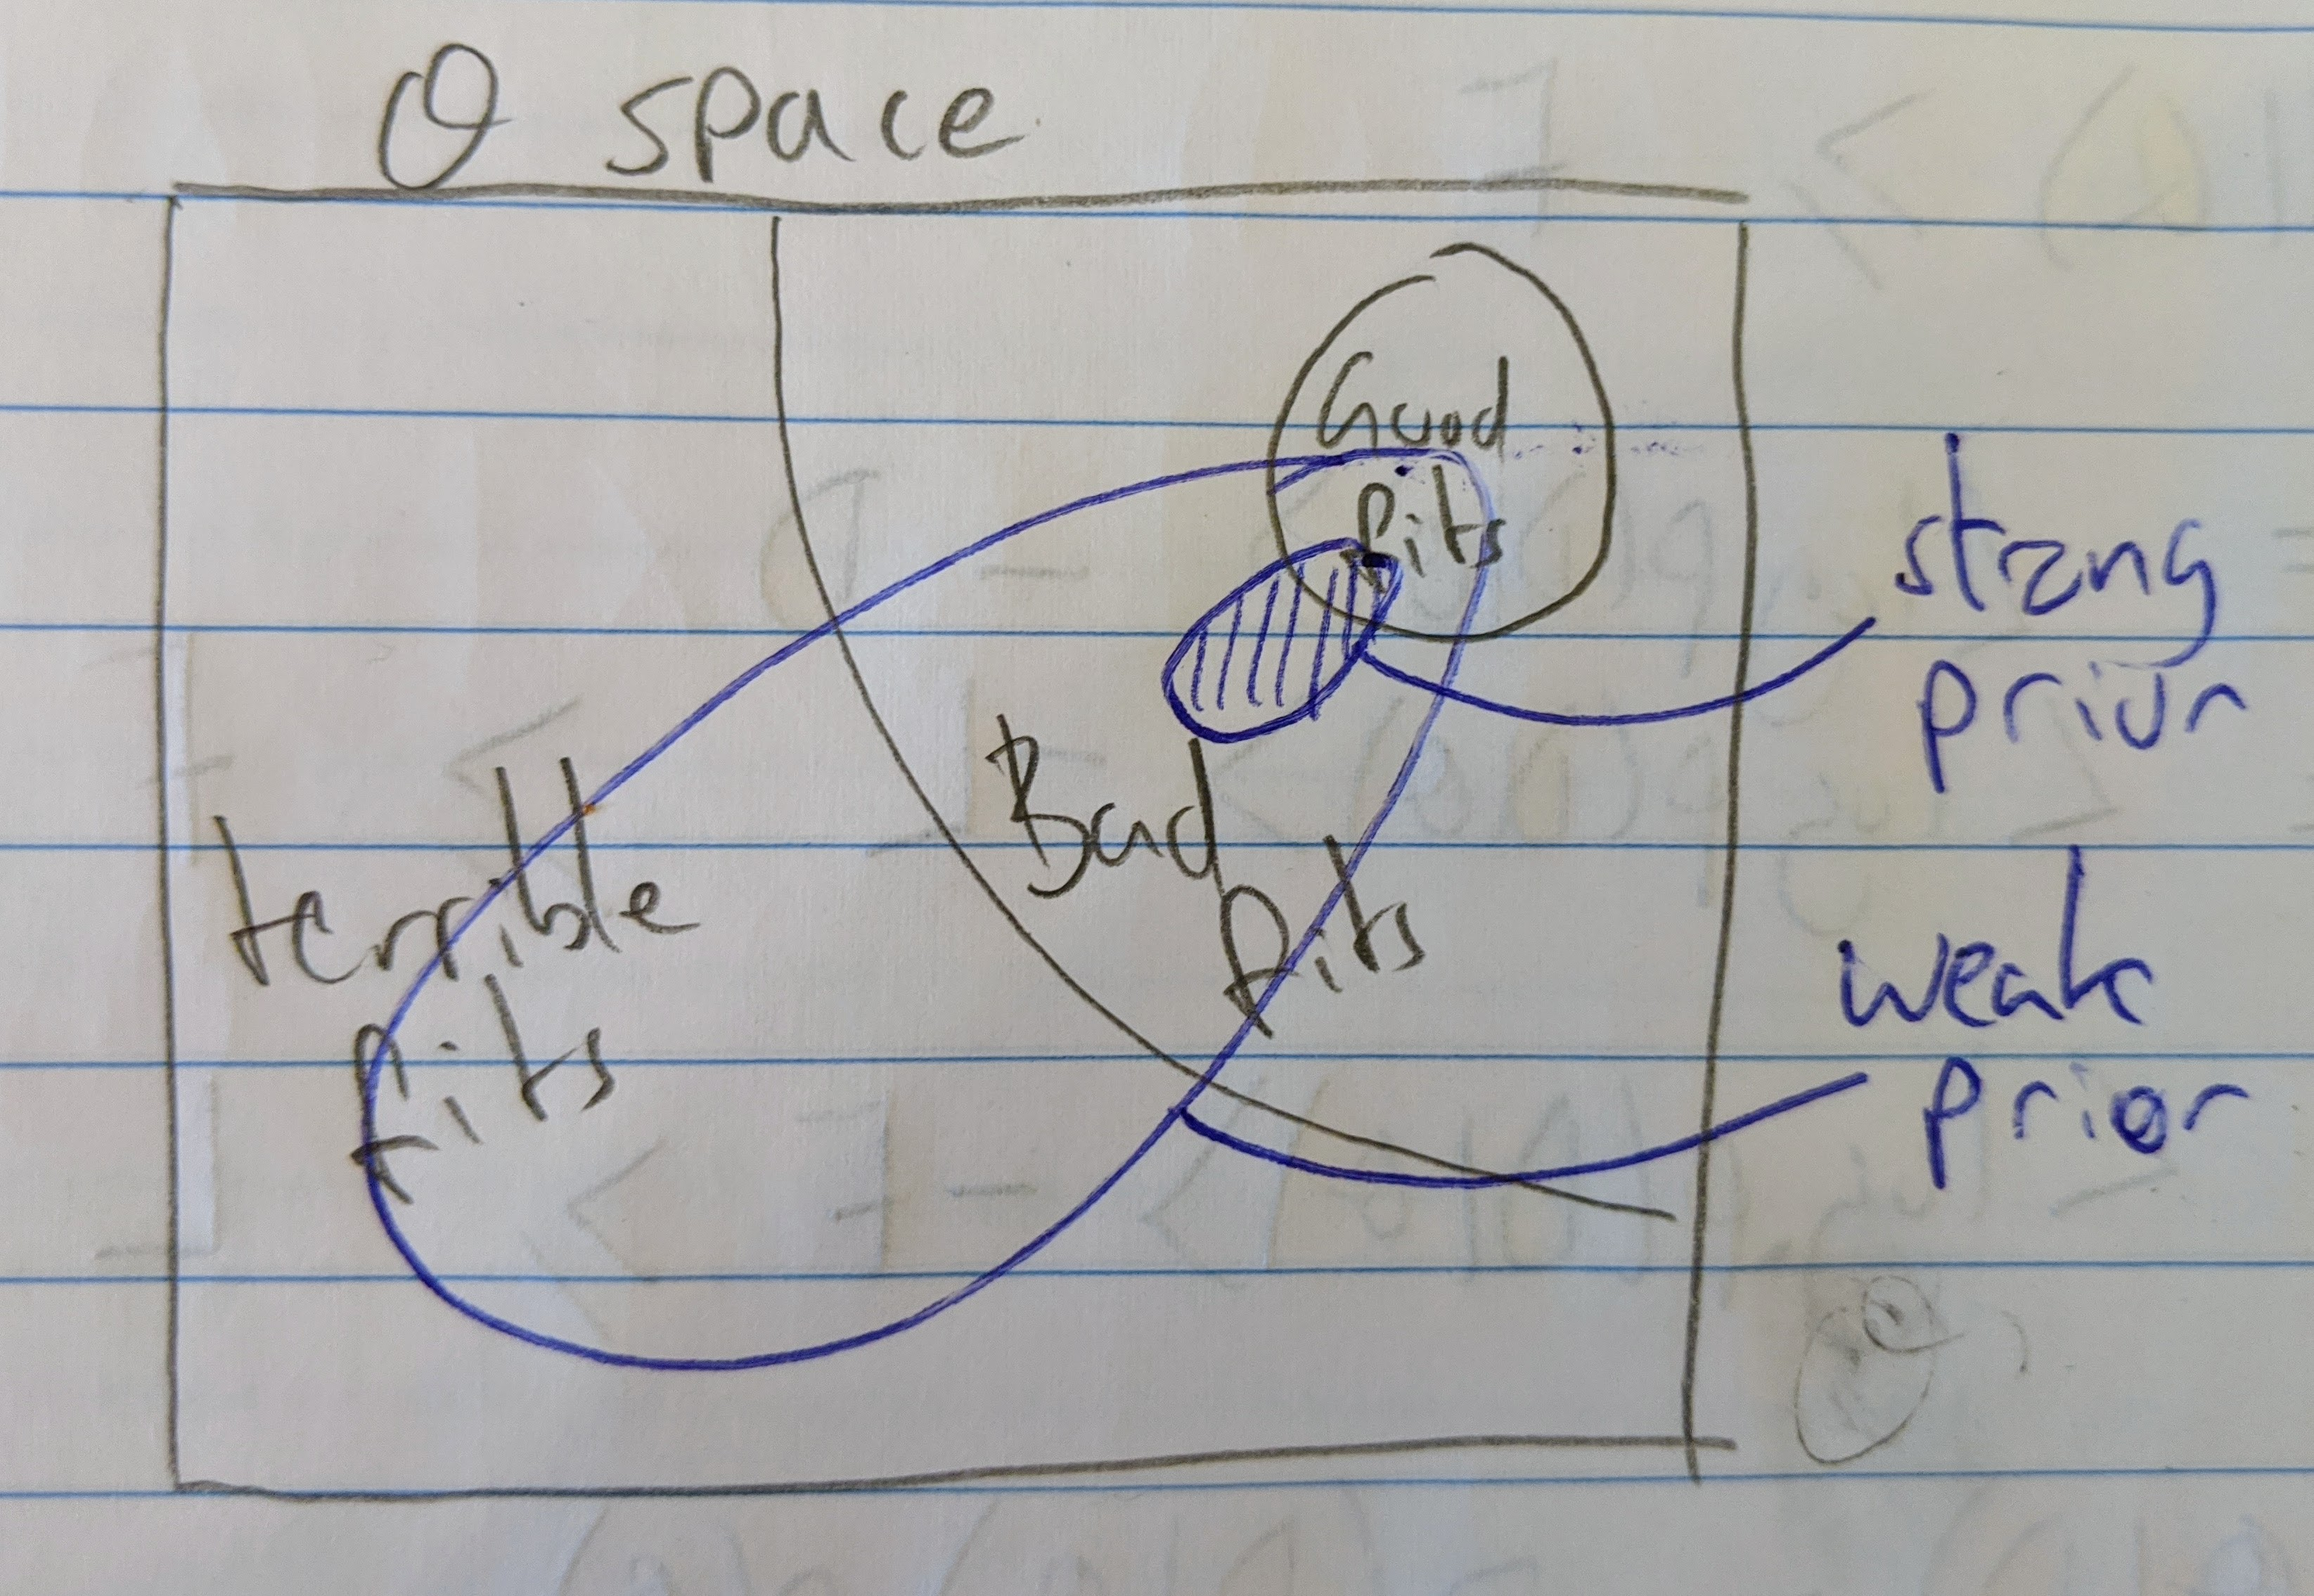
\includegraphics[width=0.5\textwidth]{lower-bound_occams-razor}
\caption{A schematic diagram of how the lower bound penalizes model complexity}
\label{fig:lb_complexity}
\end{figure}


\paragraph{Using the re-expressed marginalized likelihood, we can see the entropy forms an upper bound as well.}


\section{Experimental}
\subsection{OUTLINE Bayesian linear regression}
\subsubsection{Part 1: demonstration}
[Done except for KL divergence estimation.]
\begin{itemize}
\item The point is to test and demonstrate the accuracy of the upper and lower bounds.
\item Initialize problem with analytical priors.
\item Draw the parameters of the true data generating distribution from the prior.
\item Because the true distribution is normal, it has an analytic entropy. 
\item Show how the marginal likelihood, with lower and upper bounds evolve with increasing data.
\item Can even show the effect of improving the bounds by estimating the KL divergences.
\end{itemize}
\begin{figure}[h]
\centering
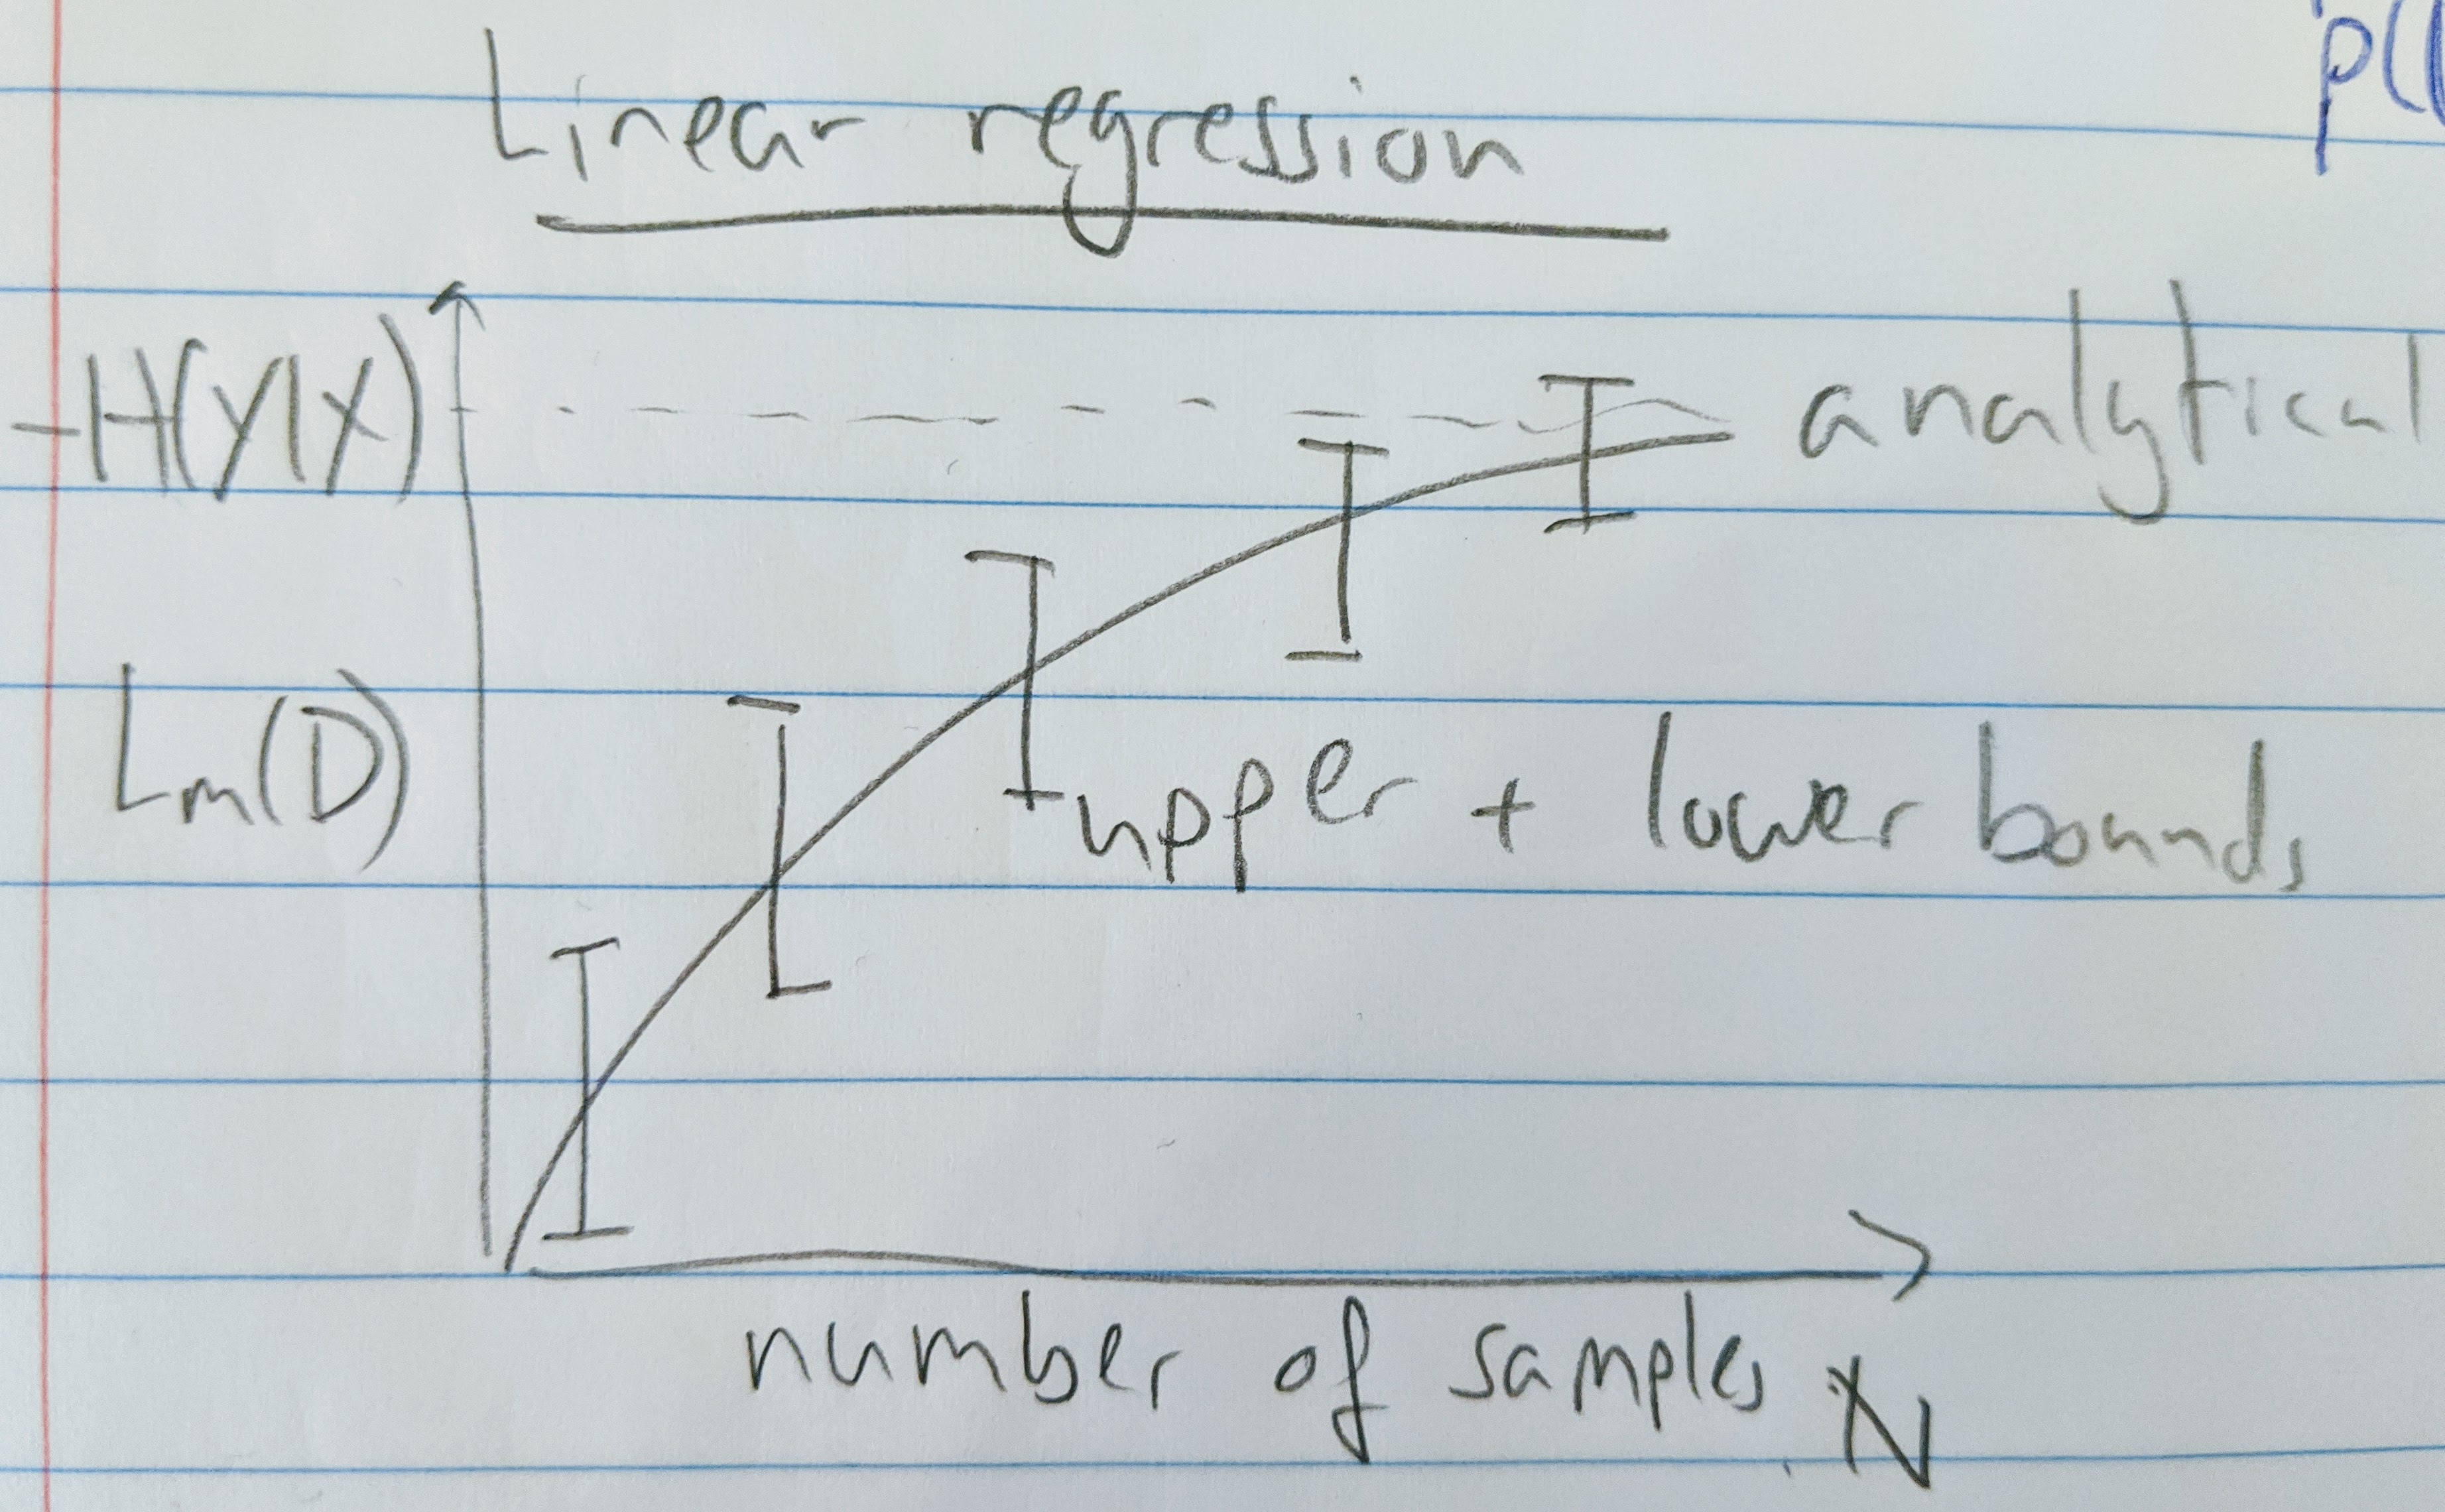
\includegraphics[width=0.5\textwidth]{expected_linregress_result}
\caption{The upper and lower bounds for Bayesian linear regression .}
\label{fig:bayes_linregress}
\end{figure}

\subsubsection{Part 2: demonstration}
Showing that the bounds are good for model selection.
\begin{itemize}
\item Automatically generate linear models with random parameters and a random number of true components and dummy components. Say 10 total variables with a chance of a variable being a true one, or varying degrees of correlated to another component.
\item Repeat many times: For increasing data points size, perform model selection to select the number of true components using a) the marginal likelihood, b) the upper bound, c) the lower bound, d) the BIC, e) the DIC, and perhaps more variants. Report the overall success rate of each technique across the repeats. 
\item Could even assess the utility of the KL divergence estimates.
\end{itemize}

\subsection{OUTLINE Model selection with Gaussian mixtures}
If my paper is about model selection I need to have at least one such numeric example here! A classic example is a mixture of Gaussians. 1D mixture is definitely easier.

\begin{itemize}
\item The entropy of a mixture of Gaussian is best approximated using Monte Carlo sampling and calculating the mean of the logarithm of density. This is guaranteed to converge to the entropy as the number of samples tends to infinity.
\item As I am approximating the marginal likelihood with bounds, I need to know the \textbf{true} marginal likelihoods (or relative difference of), or at least some gold standard reference calculation.
\item Can compare my bounded estimation of the marginal likelihood with the AIC, WAIC, and BIC in regards to picking the right number of components. These are discussed in Chapter 7 of "Bayesian Data Analysis".
\item Chapter 22 goes into a lot of depth on finite mixture models, and even has a Gibbs sampler that I can try.
\item If I can write an RJMC algorithm for guassian mixtures, then I have a "gold" standard method to estimate the marginal likelihoods. I would also have a within-model sampler. I could even use the same data to calculate the normalization ratios as well as the marginal likelihoods - I just lump all the data with the same number of components into one. 
\item See "Learning a multivariate Gaussian mixture model with the reversible jump MCMC algorithm, Zhang, Chan, and Chen, 2004".
\item Another option is non-equilibrium Monte Carlo - run MCMC with a fixed number of components, then do NCMC moves that add or remove a component. Like RJMC, I could use the within-component samples to estimate the marginal likelihoods.
\end{itemize}

\subsection{OUTLINE Model selection with neural nets}
The idea is to pick models that have a lower prediction error, rather than attempting to calculate the marginal likelihood. Model selection is over the number of hidden layers. I already have an automatic polynomial generator from my NN model.

\end{document}